\documentclass[spanish,openany]{article}
\usepackage{lmodern}
\usepackage{amssymb,amsmath}
\usepackage{ifxetex,ifluatex}
\usepackage{fixltx2e} % provides \textsubscript
\ifnum 0\ifxetex 1\fi\ifluatex 1\fi=0 % if pdftex
  \usepackage[T1]{fontenc}
  \usepackage[utf8]{inputenc}
\else % if luatex or xelatex
  \ifxetex
    \usepackage{mathspec}
  \else
    \usepackage{fontspec}
  \fi
  \defaultfontfeatures{Ligatures=TeX,Scale=MatchLowercase}
\fi
% use upquote if available, for straight quotes in verbatim environments
\IfFileExists{upquote.sty}{\usepackage{upquote}}{}
% use microtype if available
\IfFileExists{microtype.sty}{%
\usepackage{microtype}
\UseMicrotypeSet[protrusion]{basicmath} % disable protrusion for tt fonts
}{}
\usepackage[margin=1in]{geometry}
\usepackage{hyperref}
\hypersetup{unicode=true,
            pdftitle={Generación de indicadores de la vegetación de matorral seco en Alamala (Loja) a partir de imágenes multiespectrales de alta resolución},
            pdfauthor={Jesús Jiménez López},
            pdfborder={0 0 0},
            breaklinks=true}
\urlstyle{same}  % don't use monospace font for urls
\ifnum 0\ifxetex 1\fi\ifluatex 1\fi=0 % if pdftex
  \usepackage[shorthands=off,main=spanish]{babel}
\else
  \usepackage{polyglossia}
  \setmainlanguage[]{spanish}
\fi
\usepackage{natbib}
\bibliographystyle{apalike}
\usepackage{longtable,booktabs}
\usepackage{graphicx,grffile}
\makeatletter
\def\maxwidth{\ifdim\Gin@nat@width>\linewidth\linewidth\else\Gin@nat@width\fi}
\def\maxheight{\ifdim\Gin@nat@height>\textheight\textheight\else\Gin@nat@height\fi}
\makeatother
% Scale images if necessary, so that they will not overflow the page
% margins by default, and it is still possible to overwrite the defaults
% using explicit options in \includegraphics[width, height, ...]{}
\setkeys{Gin}{width=\maxwidth,height=\maxheight,keepaspectratio}
\IfFileExists{parskip.sty}{%
\usepackage{parskip}
}{% else
\setlength{\parindent}{0pt}
\setlength{\parskip}{6pt plus 2pt minus 1pt}
}
\setlength{\emergencystretch}{3em}  % prevent overfull lines
\providecommand{\tightlist}{%
  \setlength{\itemsep}{0pt}\setlength{\parskip}{0pt}}
\setcounter{secnumdepth}{5}
% Redefines (sub)paragraphs to behave more like sections
\ifx\paragraph\undefined\else
\let\oldparagraph\paragraph
\renewcommand{\paragraph}[1]{\oldparagraph{#1}\mbox{}}
\fi
\ifx\subparagraph\undefined\else
\let\oldsubparagraph\subparagraph
\renewcommand{\subparagraph}[1]{\oldsubparagraph{#1}\mbox{}}
\fi

%%% Use protect on footnotes to avoid problems with footnotes in titles
\let\rmarkdownfootnote\footnote%
\def\footnote{\protect\rmarkdownfootnote}

%%% Change title format to be more compact
\usepackage{titling}

% Create subtitle command for use in maketitle
\newcommand{\subtitle}[1]{
  \posttitle{
    \begin{center}\large#1\end{center}
    }
}

\setlength{\droptitle}{-2em}
  \title{Generación de indicadores de la vegetación de matorral seco en Alamala
(Loja) a partir de imágenes multiespectrales de alta resolución}
  \pretitle{\vspace{\droptitle}\centering\huge}
  \posttitle{\par}
  \author{Jesús Jiménez López}
  \preauthor{\centering\large\emph}
  \postauthor{\par}
  \predate{\centering\large\emph}
  \postdate{\par}
  \date{2018-03-07}

\usepackage{booktabs}
\usepackage{amsthm}
\makeatletter
\def\thm@space@setup{%
  \thm@preskip=8pt plus 2pt minus 4pt
  \thm@postskip=\thm@preskip
}
\makeatother
\usepackage{booktabs}
\usepackage{longtable}
\usepackage{array}
\usepackage{multirow}
\usepackage[table]{xcolor}
\usepackage{wrapfig}
\usepackage{float}
\usepackage{colortbl}
\usepackage{pdflscape}
\usepackage{tabu}
\usepackage{threeparttable}
\usepackage[normalem]{ulem}

\usepackage{float}

\begin{document}
\maketitle

{
\setcounter{tocdepth}{2}
\tableofcontents
}
\section*{Resumen}\label{resumen}
\addcontentsline{toc}{section}{Resumen}

Este informe describe el procedimiento empleado para la captura de
imágenes aéreas, procesamiento y cálculo de índices de vegetación a
partir de una cámara multiespectral Tetracam ADC micro instalada en un
vehículo aéreo no tripulado (RPAS, UAV). Para los vuelos en los que no
se pudieron obtener los productos fotogramétricos completos, se
seleccionaron las imágenes de mayor calidad que cubrieran las parcelas
de interés. Los resultados obtenidos demuestran que es posible generar
información multiespectral de alta resolución en áreas naturales. Sin
embargo, es preciso refinar la metodología con objeto de aumentar la
fiabilidad de los indicadores.

\section{Introducción}\label{intro}

En el campo de la teledetección ambiental se han desarrollado numerosos
cocientes e índices de vegetación relacionados con el vigor y la salud
de las plantas \citep{Bannari1995}. Estos indicadores, en conjunto con
otras métricas espectrales, han demostrado ser de gran utilidad para una
amplia variedad de estudios de ecología y conservación \citep{Wang2010}.
Desafortunadamente, las restricciones financieras y tecnológicas para la
captura de imágenes obtenidas por medio de sensores a bordo de
plataformas aéreas o espaciales han limitado la efectividad de la
teledetección en la recolección de datos de la superficie terrestre a
escalas de detalle. Como consecuencia, los RPAS se han posicionado como
un complemento adecuado para estudios ambientales en áreas de pequeña
extensión, permitiendo obtener imágenes a una elevada resolución
espacial y temporal a un menor costo \citep{Koh2012}. Este impulso ha
sido especialmente notable con el desarrollo paralelo de sensores
multiespectrales adaptados a aeronaves de pequeño tamaño, en conjunto
con la aparición de programas informáticos que facilitan el
procesamiento fotogramétrico y el análisis de grandes volúmenes de
datos.

El presente estudio investiga el uso de RPAS para estudios de vegetación
a partir del análisis de imágenes multiespectrales adquiridas durante
una campaña de vuelos en la provincia de Loja (Ecuador). Tras comentar
brevemente los índices de vegetación empleados, se describe la
metodología de campo y el procesamiento posterior de las imágenes.
Finalmente se realiza un análisis pormenorizado de los resultados
obtenidos y se proponen algunas recomendaciones de cara a futuras
campañas de vuelo.

\subsection{Índices de vegetación}\label{indices-de-vegetacion}

Los índices de vegetación (IV) son un conjunto de combinaciones
algebraicas realizadas a partir de los niveles digitales de distintas
bandas del espectro electromagnético. Han sido diseñados con objeto de
discriminar cubiertas y realzar ciertas propiedades de la vegetación
relacionadas con su composición, estructura y estado fisiológico. Estos
IV se fundamentan en el particular comportamiento radiométrico de las
plantas, dando lugar a una curva espectral típica de la vegetación
saludable {[}ver imagen \ref{fig:curvaVeg}{]}. Los pigmentos
fotosintéticos absorben la mayor parte de la radiación en el visible,
dentro del rango de la denominada radiación fotosintéticamente activa
(400 -750 µm) o PAR. Por el contrario, las hojas reflejan un gran
porcentaje de la radiación correspondiente al infrarrojo cercano
(075-1.3 µm), también denominado IRC. A medida que la vegetación enferma
la actividad fotosintética disminuye, de la misma forma que el contraste
entre ambas bandas del espectro. La caracterización de estas variaciones
de contraste constituye el fundamento de la mayoría de los IV.

\begin{center}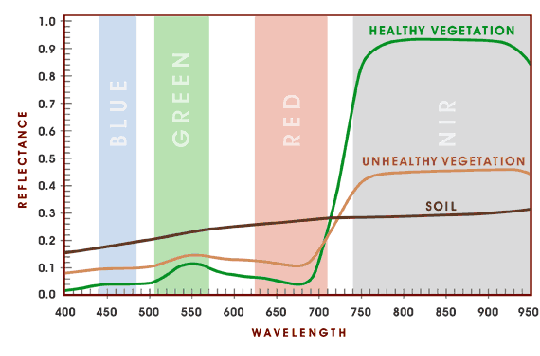
\includegraphics[width=1\linewidth]{figures/veg} \end{center}

Por regla general los IV se calculan a partir de superficies de
reflectancia, obtenidas previa calibración radiométrica de las imágenes
y teniendo en cuenta principalmente las condiciones de iluminación en el
momento de la toma, junto con otros factores dependientes de la óptica
del sensor. Si bien es posible calcular los IV directamente a partir de
los valores ``brutos'' de las imágenes, no es posible conceder un valor
físico a los resultados \citep{chuvieco2006teledeteccion}, por lo que no
son aptos para estudios cuantitativos de carácter multitemporal o en los
que se pretenda comparar los resultados obtenidos por diferentes
sensores.

En este trabajo se calcularon tres índices de vegetación (ver tabla
\ref{tab:indicesVeg}): índice de vegetación de diferencia normalizada
(NDVI), índice modificado de vegetación ajustada al suelo (MSAVI2) e
índice de vegetación de diferencia normalizada verde (GNDVI).

\begin{table}[!h]

\caption{\label{tab:indicesVeg}Índices de vegetación}
\centering
\resizebox{\linewidth}{!}{\begin{tabular}[t]{lllll}
\toprule
IV & Descripción & Fuente & Bandas & Fórmula\\
\midrule
NDVI & Normalised Difference 
 Vegetation Index & Rouse et al., 1973 & red, nir & (nir - red)/(nir + red))\\
GNDVI & Green Normalised Difference  
 Vegetation Index & Gitelson1998 & red, nir & (nir - green)/(nir + green)\\
MSAVI2 & Modified Soil Adjusted 
 Vegetation Index 2 & Qi et al., 1994 & red, nir & (2 * (nir + 1) - sqrt((2 * nir + 1)\textasciicircum{}2 - 8 * (nir - red)))/2\\
\bottomrule
\end{tabular}}
\end{table}

\subsubsection{NDVI}\label{ndvi}

El índice más conocido y más ampliamente utilizado para el monitoreo de
la vegetación es el NDVI \citep{Rouse1973}, a partir del cual han
surgido numerosas variantes. A menudo se relaciona directamente con
otros parámetros de la superficie terrestre, incluyendo el porcentaje de
cobertura del suelo, la actividad fotosintética de la planta, el
contenido de agua, el índice del área foliar y la biomasa
\citep{pettorelli2013normalized}. En otros casos ha sido empleado en
estudios que tratan de predecir patrones de biodiversidad a diferentes
escalas espaciales \citep{Madonsela2018, Gillespie2011, Levin2007}.

\subsubsection{MSAVI2}\label{msavi2}

El MSAVI2 \citep{Qi1994} aborda algunas de las limitaciones del NDVI
cuando se aplican en áreas de vegetación dispersa, con una alta
superficie de suelo desnudo. A diferencia del índice de vegetación
ajustado al suelo original (SAVI), no necesita especificar empíricamente
el factor de corrección del brillo del suelo (L) según el grado de
cobertura vegetal en el área de estudio.

\subsubsection{GNDVI}\label{gndvi}

El GNDVI \citep{Gitelson1998} es una versión modificada del NDVI,
sustituyendo la banda del rojo por la del verde. Debido a su mayor
sensibilidad a variaciones en la concentración de clorofila, ha sido
ampliamente utilizado en agricultura de precisión para caracterizar el
grado de madurez de los cultivos.

\section{Materiales y Métodos}\label{method}

\subsection{Área de estudio}\label{area-de-estudio}

El área de estudio (ver imagen \ref{fig:areaEstudio}) está situada en el
sector de Alamala, cantón de Catamayo (Loja, provincia de Ecuador). El
clima es de tipo subtropical seco, con una temperatura media anual de 27
ºC y precipitaciones de 388 mm/año. La época seca se extiende desde el
mes de mayo a enero, mientras que la temporada de lluvias abarca los
meses restantes \citep{sierra1999propuesta}. A diferencia de otras
regiones, las temperaturas más altas se registran a bajas altitudes,
suavizándose conforme se avanza a cotas más altas donde suele haber una
mayor disponibilidad de agua \citep{Espinosa2014}. El paisaje está
dominado por comunidades dispersas de matorral arbustivo sobre una
matriz de suelo desnudo, fundamentalmente por una especie del género
\emph{Croton}, perteneciente a la familia de las euforbiáceas (
\emph{Croton wagneri Mull}). En esta área se ubican las parcelas de
vegetación siguiendo un gradiente altitudinal desde los 1700 a los 1400
metros aproximadamente (según estación total). La mitad de las parcelas
consideradas están protegidas frente a la herbivoría por medio de
cercos.

\begin{figure}[H]
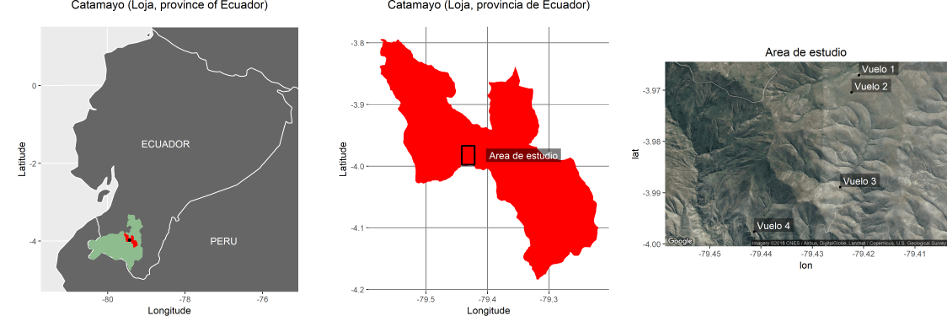
\includegraphics[width=1\linewidth,height=1\textheight]{figures/mapa_area_estudio} \caption{Área de estudio}\label{fig:areaEstudio}
\end{figure}

\subsection{Materiales empleados y operaciones de
vuelo}\label{materiales-empleados-y-operaciones-de-vuelo}

Para la toma de imágenes se utilizó un RPAS multirrotor de tipo
tetracóptero (3DR Solo), con una autonomía aproximada de 15 minutos. En
la parte inferior del RPAS se adaptó una cámara multiespectral Tetracam
ADC micro apuntando al nadir y conectada a un módulo de GPS (ver imagen
\ref{fig:camRPAS}) . Esta cámara permite obtener fotografías en falso
color (Verde, Rojo e IRC) en el rango de los 520 a 920 nanómetros,
equivalentes a Landsat TM2, TM3 y TM4. El sensor es de tipo CMOS, con
una resolución de 3.2 Megapixeles (2048 x 1536 pixeles) y presenta un
mecanismo de captura de tipo ``rolling shutter''. Los parámetros ópticos
están fijos a una distancia focal de 8,43 mm y una apertura óptica de
f/3,2.

\begin{figure}[H]
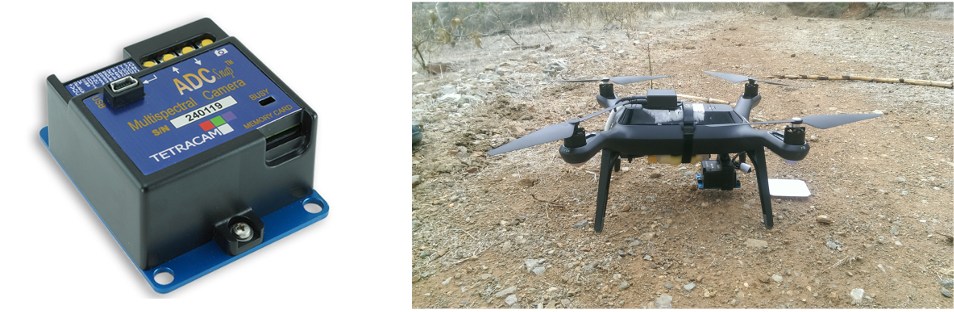
\includegraphics[width=1\linewidth,height=1\textheight]{figures/camera3drsolo} \caption{Cámara multiespectral Tetracam ADC Micro y plataforma de vuelo 3dr Solo}\label{fig:camRPAS}
\end{figure}

Cada uno de los vuelos fue diseñado con el software Mission Planner
(imagen \ref{fig:vuelos}), cubriendo las parcelas anteriormente
mencionadas y en franjas horarias comprendidas entre las 11 a.m. y las
14 a.m. horas del 13 de Diciembre de 2017 (ver tabla
\ref{tab:parcelas}). El grado de nubosidad durante este periodo pasó de
cielo prácticamente despejado a cielo parcialmente cubierto.

\begin{table}[!h]

\caption{\label{tab:parcelas}Localización de los vuelos (UTM 17S) }
\centering
\begin{tabular}[t]{rrrr}
\toprule
vuelo & este & norte & elev\\
\midrule
1 & 675316.5 & 9561342 & 1725\\
2 & 675157.2 & 9560972 & 1727\\
3 & 674904.7 & 9558930 & 1580\\
4 & 673041.8 & 9557971 & 1402\\
\bottomrule
\end{tabular}
\end{table}

El RPAS fue configurado para volar a una velocidad aproximada de 4 m/s y
a una altura media sobre el terreno de 100 metros siguiendo las misiones
previamente definidas. El periodo efectivo de vuelo se mantuvo por
debajo de los 10 minutos en todos los casos. La cámara fue programada
para la toma de imágenes cada 2 segundos aproximadamente y configurada
en ajuste automático de la velocidad de obturación, con objeto de
compensar las variaciones de iluminación en el terreno. Previamente a
cada vuelo se tomó una fotografía a un panel de calibración (teflón,
reflectancia promedio del 99\%) con objeto de calibrar radiométricamente
las imágenes.

\begin{figure}[H]
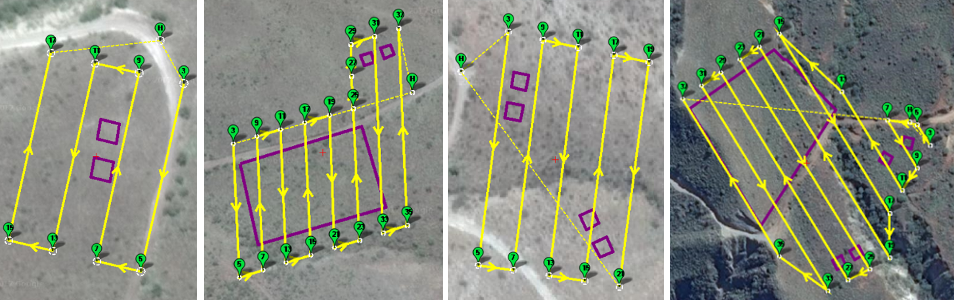
\includegraphics[width=1\linewidth,height=1\textheight]{figures/parcelas_mission_planner} \caption{Diseño de vuelos 1, 2, 3 y 4 en Mission Planner}\label{fig:vuelos}
\end{figure}

\subsection{Procesamiento de datos}\label{procesamiento-de-datos}

Las imágenes fueron procesadas mediante el software PixelWrench2 (PW2)
de Tetracam para producir composiciones en falso color mediante
interpolación cromática de los píxeles para cada una de las bandas
registradas. Inicialmente se obtuvo un archivo de coordenadas
geográficas a partir del registro generado por la cámara durante el
vuelo. Posteriormente se tomó una muestra del panel de calibración a
partir de las imágenes tomadas para cada uno de los vuelos. El archivo
de calibración generado fue utilizado para procesar las imágenes en
formato RAW, que fueron convertidas a TIFF y geoetiquetadas mediante la
programación de un script en Python \citep{Jimenez2018} que hace uso del
archivo de coordenadas generados por PW2. Posteriormente se descartaron
las imágenes que no formaban parte del plan de vuelo o consideradas de
baja calidad, según una identificación visual previa. Para generar los
mosaicos se probaron diferentes programas basados en la estructura a
partir del movimiento (SfM), incluyendo VisualSFM y versiones de prueba
de Pix4D y Agisoft Photoscan, siendo este último el elegido para el
procesamiento fotogramétrico. La mala calidad de las imágenes junto con
la ausencia de puntos de control en el terreno impidió el cálculo de los
parámetros de alineación/orientación de las escenas a partir de los
cuales se construye la nube dispersa de puntos, por lo que se optó por
seleccionar las imágenes individuales de mayor calidad que cubrieran las
parcelas de interés. Únicamente para el vuelo 3 se pudieron obtener los
productos fotogramétricos completos, incluyendo ortofoto y modelo
digital de elevaciones (DEM).

Las escenas fueron posteriormente georreferenciadas y escaladas en QGIS
\citep{QGISDevelopmentTeam2017} tomando como referencia aquellas
parcelas en las que se había instalado un cerco visible a su alrededor.
Para la corrección geométrica de las imágenes se utilizó una
transformación polinómica de primer orden, seguida de una interpolación
por convolución cúbica, recomendada para fotografías aéreas e imágenes
de satélite. A partir de las ortofotos se extrajeron las parcelas de
interés, se calcularon los índices espectrales de vegetación mediante la
libreria RStoolbox \citep{R-base, RStoolbox} y se procedió al análisis
exploratorio de los valores obtenidos. La resolución final promedio fue
de 4.5 cm/pixel, suficiente para estudios de vegetación a escala local.

\section{Resultados de los índices de vegetación}\label{results}

Debido al gran volumen de datos obtenidos, los resultados se muestran en
el \protect\hyperlink{appendix}{Anexo} adjunto. Junto con los mapas de
IV, se presentan los estadísticos más relevantes según diferentes
combinaciones de factores, incluyendo índices por parcela, gradiente
altitudinal (zonas de vuelo) e índices totales (media, mediana,
desviación típica, máximos y mínimos). Los valores obtenidos se
mantienen dentro de los límites esperados para todos los índices (-1 a
1). Valores bajos o negativos corresponden a zonas de escasa o nula
actividad fotosintética, representados en tonos amarillos a rojos. Las
zonas con presencia de vegetación aparecen en verde. EL GNDVI muestra un
comportamiento distintivo aunque coherente respecto al NDVI y MSAVI2,
probablemente por la sustitución de la banda del rojo por la del verde.

\section{Discusión y conclusiones}\label{discusion-y-conclusiones}

\subsection{Índices de vegetación}\label{indices-de-vegetacion-1}

En términos generales los IV muestran valores promedios relativamente
similares y considerablemente bajos. La baja productividad primaria
puede ser debida a la prolongada ausencia de lluvias previa a la captura
de las imágenes, dando lugar a un comportamiento más homogéneo de las
comunidades vegetales independientemente de su ubicación. Sería
interesante comparar los resultados frente a condiciones climáticas más
benignas, caracterizadas por periodos de relativa abundancia de agua y
probablemente menor insolación. La desviación típica refleja la
variabilidad espacial en la productividad de los ecosistemas y no parece
verse afectada en exceso por valores extremos. La presencia de picos
máximos en los IV suele estar relacionada con áreas de vegetación donde
la actividad fotosintética es más acusada, si bien la baja densidad de
valores particularmente altos podría reflejar una deficiente calibración
del sensor. Un análisis estadístico apropiado de los datos obtenidos
permitiría evaluar posibles cambios en la cobertura vegetal y actividad
fotosintética de las plantas en función del gradiente altitudinal y la
presencia / ausencia de herbivoría. Estas diferencias podrían ser más
marcadas en temporada de lluvias. Para analizar estas diferencias y
obtener resultados más concluyentes convendría ampliar el rango temporal
del estudio.

\subsection{Limitaciones del sensor y consideraciones de
vuelo}\label{limitaciones-del-sensor-y-consideraciones-de-vuelo}

La cámara multiespectral Tetracam ADC micro tiene algunas limitaciones
técnicas importantes que conviene aclarar. El sensor de banda ancha está
diseñado a partir de una matriz simple de fotodiodos, denominada matriz
de Bayer, sensibles a cambios en la intensidad lumínica. Estos
fotodiodos no son capaces de discriminar el color, por lo que
generalmente se procede a una interpolación de los valores obtenidos
según la disposición de un conjunto de filtros selectivos que en
principio solo dejan pasar la radiación para cada uno de los tres
canales disponibles. Esta configuración es habitual en la mayoría de
cámaras de consumo, pero generalmente adolecen de un mayor solape
espectral entre bandas. La mezcla de la señal para diferentes longitudes
de onda dificulta en gran medida la discriminación de la respuesta
espectral de la vegetación y la comparación con otros sensores de alta
gama. Por otra parte, la cámara utiliza un mecanismo de captura de tipo
``rolling shutter'', por el cual la imagen se registra siguiendo un
proceso secuencial de escaneado en sentido vertical u horizontal. Este
sistema suele ser propenso a una serie de distorsiones en la imagen
cuando la fotografía se realiza desde plataformas móviles que se
desplazan con relativa rapidez (imagen \ref{fig:rolling}). En este
estudio, las imágenes están severamente afectadas por este fenómeno,
imposibilitando la identificación de puntos homólogos entre imágenes y
por tanto la adecuada optimización de los parámetros de calibración para
cada una de las tomas aéreas, condición previa al procesamiento
fotogramétrico.

\begin{figure}
\includegraphics[width=1\linewidth]{figures/TTC08236} \caption{Efecto típico rolling shutter}\label{fig:rolling}
\end{figure}

Para minimizar el efecto rolling shutter lo más apropiado es emplear
algún sistema estabilizador de la cámara que pueda amortiguar las
vibraciones propias del RPAS y corregir las oscilaciones de la
plataforma con objeto de mantener el sensor en posición perpendicular
respecto a la superficie de estudio. Adicionalmente conviene calibrar
adecuadamente el RPAS y optimizar el plan de vuelo. En este sentido, la
velocidad y la altura de vuelo son los factores más importantes a tener
en cuenta. Una mayor altura podría reducir teóricamente los artefactos
típicos del rolling shutter, además de acortar los tiempos de vuelo en
detrimento de una menor resolución espacial. Sin embargo, hay que tener
en cuenta las restricciones legales que impiden volar por encima de una
altura superior a los 122 metros en Ecuador. Por otro lado, una menor
velocidad de vuelo aumentaría considerablemente los tiempos de la
operación, aunque incidiría positivamente en la calidad de las imágenes.
En cualquier caso, para parcelas de pequeño tamaño, podría ser adecuado
realizar un sobrevuelo perpendicular a la zona de estudio. La altura de
vuelo requerida para cubrir completamente la zona de estudio es
fácilmente calculable a partir del ángulo de visión (FOV) de la cámara.
Este planteamiento es fácilmente implementable, menos arriesgado y
requiere un menor despliegue de recursos.

\subsection{Calibración geométrica}\label{calibracion-geometrica}

El error cuadrático medio durante la fase de georreferenciación se situó
por debajo de los 40 píxeles por escena, salvo para el vuelo 3, en el
que debido a la mayor superficie a georreferenciar y la inadecuada
distribución de los puntos de control, el error reportado fue mayor.
Este error se mantuvo relativamente constante en todos los puntos para
cada parcela y no debe afectar el cálculo de los índices, por lo que no
se consideró necesario optimizar la georreferenciación. Sin embargo hay
que tener en cuenta que los IV fueron calculados a partir de imágenes
individuales, debido a la imposibilidad para generar los mosaicos. Por
tanto, es de esperar que el procesamiento fotogramétrico de las imágenes
mejoraría drásticamente por medio del uso de dianas adecuadamente
distribuidas por el terreno y correctamente posicionadas mediante GPS
diferencial o estación total. Esto es particularmente importante fuera
de áreas urbanas, donde suele ser más complicado identificar puntos
homólogos entre imágenes.

\subsection{Calibración radiométrica}\label{calibracion-radiometrica}

El cálculo de reflectividades es especialmente importante cuando se
trabaja en diferentes condiciones de iluminación, fechas o sensores, por
lo que la mejora en el procedimiento de calibración radiométrica de las
imágenes debería ser una de las necesidades prioritarias en estudios de
vegetación. En caso contrario los IV deben ser interpretados
cualitativamente. En términos generales, sería recomendable usar valores
de exposición fijos durante toda la operación y en función de las
condiciones de iluminación in situ, con objeto de facilitar la
calibración radiométrica. El uso de paneles de calibración con
reflectividades conocidas permitiría aproximar los niveles digitales de
las imágenes a valores físicos de reflectancia, siguiendo alguno de los
procedimientos establecidos en otros estudios. Por lo general el método
lineal de calibración empírica \citep{Smith1999} suele dar resultados
aceptables y es el más ampliamente utilizado. En este estudio se utilizó
una muestra de los niveles digitales obtenidos a partir de una placa de
teflón fotografiada con anterioridad a cada vuelo. Para obtener una
muestra suficiente es necesario que la placa cubra la mayor parte de la
imagen y que no aparezca sobreexpuesta. En nuestro estudio no se
cumplieron ninguno de los dos requisitos. En cualquier caso, este
procedimiento serviría únicamente para aproximar valores de reflectancia
relativa, comparables a lo sumo para índices generados en un mismo día.
Actualmente la calibración radiométrica de las imágenes obtenidas
mediante RPAS está en fase constante de investigación. La aparición de
una nueva generación de sensores multiespectrales y paneles de
calibración adecuados proporcionan una mayor solidez a los resultados.

\subsection*{Agradecimientos}\label{agradecimientos}
\addcontentsline{toc}{subsection}{Agradecimientos}

Agradecimientos por el apoyo recibido en los trabajos de campo al
personal de la Universidad Técnica Particular de Loja (UTPL) y la
empresa Kea Electronics.

\hypertarget{appendix}{\section{Anexo}\label{appendix}}

\subsection{Estadísticos}\label{estadisticos}

\begin{table}[!h]

\caption{\label{tab:unnamed-chunk-2}Índices de vegetación totales}
\centering
\begin{tabular}[t]{lrrrrr}
\toprule
ind & mean & median & max & min & sd\\
\midrule
NDVI & 0.1396795 & 0.1369355 & 0.7888946 & -0.4423651 & 0.0734385\\
MSAVI2 & 0.2379044 & 0.2408821 & 0.8819896 & -1.5864547 & 0.1126259\\
GNDVI & 0.0193508 & 0.0193178 & 0.3138509 & -0.3307167 & 0.0486787\\
\bottomrule
\end{tabular}
\end{table}

\begin{table}[!h]

\caption{\label{tab:unnamed-chunk-3}Índices de vegetación por gradiente altitudinal (vuelos) }
\centering
\begin{tabular}[t]{lrrrrrr}
\toprule
ind & flight & mean & median & max & min & sd\\
\midrule
NDVI & 1 & 0.1296670 & 0.1271370 & 0.7888946 & -0.4423651 & 0.0759787\\
NDVI & 2 & 0.1572704 & 0.1565326 & 0.5979065 & -0.2354898 & 0.0658281\\
NDVI & 3 & 0.1213978 & 0.1181474 & 0.7040910 & -0.1409042 & 0.0729591\\
NDVI & 4 & 0.1553812 & 0.1534823 & 0.5798342 & -0.2199263 & 0.0708295\\
MSAVI2 & 1 & 0.2215505 & 0.2255901 & 0.8819896 & -1.5864547 & 0.1200708\\
\addlinespace
MSAVI2 & 2 & 0.2661634 & 0.2706892 & 0.7483582 & -0.6160308 & 0.0993437\\
MSAVI2 & 3 & 0.2093114 & 0.2113234 & 0.8263518 & -0.3280206 & 0.1115663\\
MSAVI2 & 4 & 0.2624435 & 0.2661170 & 0.7340420 & -0.5638444 & 0.1067918\\
GNDVI & 1 & 0.0390770 & 0.0394827 & 0.3138509 & -0.3307167 & 0.0470861\\
GNDVI & 2 & 0.0128789 & 0.0133204 & 0.2114307 & -0.2318848 & 0.0430949\\
\addlinespace
GNDVI & 3 & 0.0033402 & 0.0035652 & 0.2530240 & -0.2008531 & 0.0471353\\
GNDVI & 4 & 0.0282264 & 0.0293981 & 0.2429195 & -0.2472101 & 0.0481237\\
\bottomrule
\end{tabular}
\end{table}

\begin{table}[!h]

\caption{\label{tab:unnamed-chunk-4}Índices de vegetación por parcelas}
\centering
\begin{tabular}[t]{llrrrrr}
\toprule
ind & .id & mean & median & max & min & sd\\
\midrule
NDVI & p11 & 0.1115298 & 0.1093149 & 0.6789593 & -0.3911617 & 0.0705064\\
NDVI & p12 & 0.1477596 & 0.1456597 & 0.7888946 & -0.4423651 & 0.0769219\\
NDVI & p21 & 0.1616221 & 0.1607373 & 0.5979065 & -0.2049998 & 0.0640664\\
NDVI & p22 & 0.1528952 & 0.1518418 & 0.5271614 & -0.2354898 & 0.0672702\\
NDVI & p31 & 0.1246447 & 0.1205831 & 0.5724941 & -0.1276600 & 0.0739729\\
\addlinespace
NDVI & p32 & 0.1242078 & 0.1135236 & 0.7040910 & -0.1409042 & 0.0923983\\
NDVI & p33 & 0.1274104 & 0.1277553 & 0.4663089 & -0.1128611 & 0.0573718\\
NDVI & p34 & 0.1092773 & 0.1095825 & 0.5516765 & -0.1129146 & 0.0592624\\
NDVI & p41 & 0.1662771 & 0.1688380 & 0.4901818 & -0.2045846 & 0.0694682\\
NDVI & p42 & 0.1964815 & 0.1972639 & 0.5798342 & -0.0779372 & 0.0653344\\
\addlinespace
NDVI & p43 & 0.1368097 & 0.1349256 & 0.5217252 & -0.2000914 & 0.0609464\\
NDVI & p44 & 0.1123248 & 0.1106322 & 0.3985167 & -0.2199263 & 0.0555369\\
MSAVI2 & p11 & 0.1934562 & 0.1970827 & 0.8087823 & -1.2848808 & 0.1145325\\
MSAVI2 & p12 & 0.2495756 & 0.2542776 & 0.8819896 & -1.5864547 & 0.1189139\\
MSAVI2 & p21 & 0.2729907 & 0.2769535 & 0.7483582 & -0.5157088 & 0.0960530\\
\addlinespace
MSAVI2 & p22 & 0.2592993 & 0.2636461 & 0.6903772 & -0.6160308 & 0.1020873\\
MSAVI2 & p31 & 0.2142975 & 0.2152112 & 0.7281318 & -0.2926750 & 0.1127622\\
MSAVI2 & p32 & 0.2099254 & 0.2038969 & 0.8263518 & -0.3280206 & 0.1358011\\
MSAVI2 & p33 & 0.2214214 & 0.2265616 & 0.6360270 & -0.2544299 & 0.0906675\\
MSAVI2 & p34 & 0.1918564 & 0.1975166 & 0.7110690 & -0.2545668 & 0.0969995\\
\addlinespace
MSAVI2 & p41 & 0.2789359 & 0.2888951 & 0.6578782 & -0.5143943 & 0.1045245\\
MSAVI2 & p42 & 0.3233867 & 0.3295206 & 0.7340420 & -0.1690460 & 0.0926396\\
MSAVI2 & p43 & 0.2356386 & 0.2377674 & 0.6856991 & -0.5002749 & 0.0945126\\
MSAVI2 & p44 & 0.1974773 & 0.1992206 & 0.5699077 & -0.5638444 & 0.0900616\\
GNDVI & p11 & 0.0266924 & 0.0268910 & 0.3138509 & -0.2242873 & 0.0469408\\
\addlinespace
GNDVI & p12 & 0.0514311 & 0.0512642 & 0.2593017 & -0.3307167 & 0.0438763\\
GNDVI & p21 & 0.0191072 & 0.0197479 & 0.2114307 & -0.2318848 & 0.0424443\\
GNDVI & p22 & 0.0066170 & 0.0067354 & 0.2033380 & -0.1685503 & 0.0428361\\
GNDVI & p31 & 0.0148962 & 0.0149040 & 0.2368022 & -0.1915286 & 0.0432251\\
GNDVI & p32 & 0.0216830 & 0.0211112 & 0.2530240 & -0.1876830 & 0.0481303\\
\addlinespace
GNDVI & p33 & -0.0014523 & -0.0011751 & 0.1825909 & -0.1825140 & 0.0403691\\
GNDVI & p34 & -0.0231511 & -0.0222579 & 0.1916022 & -0.2008531 & 0.0428077\\
GNDVI & p41 & 0.0507431 & 0.0512225 & 0.2108868 & -0.1413049 & 0.0406018\\
GNDVI & p42 & 0.0511864 & 0.0516566 & 0.2429195 & -0.1905495 & 0.0390907\\
GNDVI & p43 & 0.0122107 & 0.0118657 & 0.2034398 & -0.2472101 & 0.0435647\\
GNDVI & p44 & -0.0096494 & -0.0101914 & 0.1588499 & -0.1889714 & 0.0392273\\
\bottomrule
\end{tabular}
\end{table}

\subsection{Ortomosaicos}\label{ortomosaicos}

\subsubsection{Vuelo 1}\label{vuelo-1}

\includegraphics[width=0.33\linewidth]{../post-processing/parcela1/5_analysis/figures/parcela1}
\includegraphics[width=0.33\linewidth]{../post-processing/parcela1/5_analysis/figures/parcela1_1}
\includegraphics[width=0.33\linewidth]{../post-processing/parcela1/5_analysis/figures/parcela1_2}

\subsubsection{Vuelo 2}\label{vuelo-2}

\includegraphics[width=0.33\linewidth]{../post-processing/parcela2/5_analysis/figures/parcela2}
\includegraphics[width=0.33\linewidth]{../post-processing/parcela2/5_analysis/figures/parcela2_1}
\includegraphics[width=0.33\linewidth]{../post-processing/parcela2/5_analysis/figures/parcela2_2}

\subsubsection{Vuelo 3}\label{vuelo-3}

\includegraphics[width=0.33\linewidth]{../post-processing/parcela3/5_analysis/figures/parcela3}
\includegraphics[width=0.33\linewidth]{../post-processing/parcela3/5_analysis/figures/parcela3_1}
\includegraphics[width=0.33\linewidth]{../post-processing/parcela3/5_analysis/figures/parcela3_2}
\includegraphics[width=0.33\linewidth]{../post-processing/parcela3/5_analysis/figures/parcela3_3}
\includegraphics[width=0.33\linewidth]{../post-processing/parcela3/5_analysis/figures/parcela3_4}

\subsubsection{Vuelo 4}\label{vuelo-4}

\includegraphics[width=0.33\linewidth]{../post-processing/parcela4/5_analysis/figures/parcela4N}
\includegraphics[width=0.33\linewidth]{../post-processing/parcela4/5_analysis/figures/parcela4_1}
\includegraphics[width=0.33\linewidth]{../post-processing/parcela4/5_analysis/figures/parcela4_2}

\includegraphics[width=0.33\linewidth]{../post-processing/parcela4/5_analysis/figures/parcela4S}
\includegraphics[width=0.33\linewidth]{../post-processing/parcela4/5_analysis/figures/parcela4_3}
\includegraphics[width=0.33\linewidth]{../post-processing/parcela4/5_analysis/figures/parcela4_4}

\subsection{Índices de vegetación}\label{indices-de-vegetacion-2}

\subsubsection{Vuelo 1}\label{vuelo-1-1}

\includegraphics[width=0.33\linewidth]{../post-processing/parcela1/5_analysis/figures/parcela1_1_NDVI}
\includegraphics[width=0.33\linewidth]{../post-processing/parcela1/5_analysis/figures/parcela1_1_GNDVI}
\includegraphics[width=0.33\linewidth]{../post-processing/parcela1/5_analysis/figures/parcela1_1_MSAVI2}

\includegraphics[width=0.33\linewidth]{../post-processing/parcela1/5_analysis/figures/parcela1_2_NDVI}
\includegraphics[width=0.33\linewidth]{../post-processing/parcela1/5_analysis/figures/parcela1_2_GNDVI}
\includegraphics[width=0.33\linewidth]{../post-processing/parcela1/5_analysis/figures/parcela1_2_MSAVI2}

\includegraphics[width=0.33\linewidth]{../post-processing/parcela1/5_analysis/figures/boxplot_p11_p12_NDVI}
\includegraphics[width=0.33\linewidth]{../post-processing/parcela1/5_analysis/figures/boxplot_p11_p12_GNDVI}
\includegraphics[width=0.33\linewidth]{../post-processing/parcela1/5_analysis/figures/boxplot_p11_p12_MSAVI2}

\includegraphics[width=0.33\linewidth]{../post-processing/parcela1/5_analysis/figures/histo_p11_p12_NDVI}
\includegraphics[width=0.33\linewidth]{../post-processing/parcela1/5_analysis/figures/histo_p11_p12_GNDVI}
\includegraphics[width=0.33\linewidth]{../post-processing/parcela1/5_analysis/figures/histo_p11_p12_MSAVI2}

\subsubsection{Vuelo 2}\label{vuelo-2-1}

\includegraphics[width=0.33\linewidth]{../post-processing/parcela2/5_analysis/figures/parcela2_1_NDVI}
\includegraphics[width=0.33\linewidth]{../post-processing/parcela2/5_analysis/figures/parcela2_1_GNDVI}
\includegraphics[width=0.33\linewidth]{../post-processing/parcela2/5_analysis/figures/parcela2_1_MSAVI2}

\includegraphics[width=0.33\linewidth]{../post-processing/parcela2/5_analysis/figures/parcela2_2_NDVI}
\includegraphics[width=0.33\linewidth]{../post-processing/parcela2/5_analysis/figures/parcela2_2_GNDVI}
\includegraphics[width=0.33\linewidth]{../post-processing/parcela2/5_analysis/figures/parcela2_2_MSAVI2}

\includegraphics[width=0.33\linewidth]{../post-processing/parcela2/5_analysis/figures/boxplot_p21_p22_NDVI}
\includegraphics[width=0.33\linewidth]{../post-processing/parcela2/5_analysis/figures/boxplot_p21_p22_GNDVI}
\includegraphics[width=0.33\linewidth]{../post-processing/parcela2/5_analysis/figures/boxplot_p21_p22_MSAVI2}

\includegraphics[width=0.33\linewidth]{../post-processing/parcela2/5_analysis/figures/histo_p21_p22_NDVI}
\includegraphics[width=0.33\linewidth]{../post-processing/parcela2/5_analysis/figures/histo_p21_p22_GNDVI}
\includegraphics[width=0.33\linewidth]{../post-processing/parcela2/5_analysis/figures/histo_p21_p22_MSAVI2}

\subsubsection{Vuelo 3}\label{vuelo-3-1}

\includegraphics[width=0.33\linewidth]{../post-processing/parcela3/5_analysis/figures/parcela3_1_NDVI}
\includegraphics[width=0.33\linewidth]{../post-processing/parcela3/5_analysis/figures/parcela3_1_GNDVI}
\includegraphics[width=0.33\linewidth]{../post-processing/parcela3/5_analysis/figures/parcela3_1_MSAVI2}

\includegraphics[width=0.33\linewidth]{../post-processing/parcela3/5_analysis/figures/parcela3_2_NDVI}
\includegraphics[width=0.33\linewidth]{../post-processing/parcela3/5_analysis/figures/parcela3_2_GNDVI}
\includegraphics[width=0.33\linewidth]{../post-processing/parcela3/5_analysis/figures/parcela3_2_MSAVI2}

\includegraphics[width=0.33\linewidth]{../post-processing/parcela3/5_analysis/figures/parcela3_3_NDVI}
\includegraphics[width=0.33\linewidth]{../post-processing/parcela3/5_analysis/figures/parcela3_3_GNDVI}
\includegraphics[width=0.33\linewidth]{../post-processing/parcela3/5_analysis/figures/parcela3_3_MSAVI2}

\includegraphics[width=0.33\linewidth]{../post-processing/parcela3/5_analysis/figures/parcela3_4_NDVI}
\includegraphics[width=0.33\linewidth]{../post-processing/parcela3/5_analysis/figures/parcela3_4_GNDVI}
\includegraphics[width=0.33\linewidth]{../post-processing/parcela3/5_analysis/figures/parcela3_4_MSAVI2}

\includegraphics[width=0.33\linewidth]{../post-processing/parcela3/5_analysis/figures/boxplot_p31_p32_p33_p34_NDVI}
\includegraphics[width=0.33\linewidth]{../post-processing/parcela3/5_analysis/figures/boxplot_p31_p32_p33_p34_GNDVI}
\includegraphics[width=0.33\linewidth]{../post-processing/parcela3/5_analysis/figures/boxplot_p31_p32_p33_p34_MSAVI2}

\includegraphics[width=0.33\linewidth]{../post-processing/parcela3/5_analysis/figures/histo_p31_p32_p33_p34_NDVI}
\includegraphics[width=0.33\linewidth]{../post-processing/parcela3/5_analysis/figures/histo_p31_p32_p33_p34_GNDVI}
\includegraphics[width=0.33\linewidth]{../post-processing/parcela3/5_analysis/figures/histo_p31_p32_p33_p34_MSAVI2}

\subsubsection{Vuelo 4}\label{vuelo-4-1}

\includegraphics[width=0.33\linewidth]{../post-processing/parcela4/5_analysis/figures/parcela4_1_NDVI}
\includegraphics[width=0.33\linewidth]{../post-processing/parcela4/5_analysis/figures/parcela4_1_GNDVI}
\includegraphics[width=0.33\linewidth]{../post-processing/parcela4/5_analysis/figures/parcela4_1_MSAVI2}

\includegraphics[width=0.33\linewidth]{../post-processing/parcela4/5_analysis/figures/parcela4_2_NDVI}
\includegraphics[width=0.33\linewidth]{../post-processing/parcela4/5_analysis/figures/parcela4_2_GNDVI}
\includegraphics[width=0.33\linewidth]{../post-processing/parcela4/5_analysis/figures/parcela4_2_MSAVI2}

\includegraphics[width=0.33\linewidth]{../post-processing/parcela4/5_analysis/figures/parcela4_3_NDVI}
\includegraphics[width=0.33\linewidth]{../post-processing/parcela4/5_analysis/figures/parcela4_3_GNDVI}
\includegraphics[width=0.33\linewidth]{../post-processing/parcela4/5_analysis/figures/parcela4_3_MSAVI2}

\includegraphics[width=0.33\linewidth]{../post-processing/parcela4/5_analysis/figures/parcela4_4_NDVI}
\includegraphics[width=0.33\linewidth]{../post-processing/parcela4/5_analysis/figures/parcela4_4_GNDVI}
\includegraphics[width=0.33\linewidth]{../post-processing/parcela4/5_analysis/figures/parcela4_4_MSAVI2}

\includegraphics[width=0.33\linewidth]{../post-processing/parcela4/5_analysis/figures/boxplot_p41_p42_p43_p44_NDVI}
\includegraphics[width=0.33\linewidth]{../post-processing/parcela4/5_analysis/figures/boxplot_p41_p42_p43_p44_GNDVI}
\includegraphics[width=0.33\linewidth]{../post-processing/parcela4/5_analysis/figures/boxplot_p41_p42_p43_p44_MSAVI2}

\includegraphics[width=0.33\linewidth]{../post-processing/parcela4/5_analysis/figures/histo_p41_p42_p43_p44_NDVI}
\includegraphics[width=0.33\linewidth]{../post-processing/parcela4/5_analysis/figures/histo_p41_p42_p43_p44_GNDVI}
\includegraphics[width=0.33\linewidth]{../post-processing/parcela4/5_analysis/figures/histo_p41_p42_p43_p44_MSAVI2}

\bibliography{book.bib,packages.bib,references.bib}


\end{document}
